\chapter{Introduction}\label{ch:intro}

Human cognition relies on the ability to sense, process, and understand the surrounding environment and its sounds.
Although the skill of listening and understanding their origin is so natural for living beings, it still results in a very challenging task for computers. In recent years several novel methods have been proposed to analyze this information automatically, and several new applications have emerged \cite{virtanen2018computational}. However, the creation of ``machine listening'' algorithms that can mimic this cognitive feature by means of artificial systems remains a very challenging task. 

Nowdays, one of the main subject of interest in technological research regards systems deployed for surveillance applications. Surveillance can be seen as control of public safety or as the supervision of private environments where people may live alone. 
In fact, the increasing level of public security over the past decades has motivated the installation of sensors such as cameras or microphones in public places (stores, subway, airports, etc.), while is possible to effectively consider personal multimedia devices (smartphones, tablets, etc.) as virtual assistant which is able to monitor the user and eventually intervene in case of necessity without having the need for a physical interface (i.e., keyboard) anymore.
Thus, the need of unsupervised situation assessment stimulated the signal processing community towards experimenting with several automated frameworks, due to their potential in several engineering applications.

In these contexts, sound or sound sensing can be advantageous with respect to other modalities of multimedia processing.  
This is the case of acoustic surveillance \cite{crocco2016audio}, healthcare monitoring \cite{peng2009healthcare, foggia2015reliable} or urban sound analysis \cite{salamon2017deep}, where the short duration of certain events (i.e., a human fall, a gunshot or a glass breaking) or the personal privacy motivate the exploitation of the audio information rather than, e.g., the image processing. 
In addition, audio processing is often less computationally demanding compared to other multimedia domains, thus embedded devices can be easily equipped with microphones and sufficient computational capacity to locally process the signal captured. 
These could be smart home devices for home automation purposes or sensors for wildlife and biodiversity monitoring (i.e., bird calls detection \cite{grill2017two}). 
Some of these applications have already become commercial products that are able recognize certain specific sound categories in realistic environments and improve home security \cite{audioanalytic}  or companies with as much impactful missions, such as preserve the Rainforest from illegal deforestation \cite{rainforest}.

The type of information to be extracted with these algorithms depends on the application. In particular, we can sort the sound analysis tasks explored in this work into two high-level categories: sound event \textit{detection} and sound event \textit{classification}.
In sound event detection (SED), or acoustic event detection, the goal is to detect the onset and offset times for a variety of sound events captured in an audio recording. 

In sound event classification, the goal is to categorize an audio recording into one of a set of predefined categories by associating a textual descriptor.

In controlled laboratory conditions where the data used to develop computational sound scene and event analysis methods matches well with the test data, it is possible to achieve relatively high accuracies in the detection and classification of sounds.  However, there are several complexities in computational sound analysis and current technologies face many challenges, mainly related to the acoustics of sound scenes and events, when they are employed in realistic environments.
Among these challenges we can include:
\begin{itemize}
	\item the effect of the environment acoustics: reverberation, background noises and the channel coupling (impulse response) between the source and the recording equipment;
	\item the intra-class variability, i.e., high difference of the acoustic characteristics of even a single class of sounds and on the other hand the similarity of many different types of sounds to the target events  \cite{stowell2015acoustic};
	\item the \textit{polyphony}, i.e. the occurrence of multiple simultaneous events. In realistic environments there
are almost always multiple sources producing sound at the same time. 
\end{itemize}

In addition to these complications related to the acoustics of sound scenes and
events, there are also several fundamental limitations related to the computational methods. In particular, to develop effective models based on the \textit{deep learning} paradigm, a very large set of examples of the
target (and non-target) sounds is required. In contrast to the situation in image classification,
 currently available datasets that can be used to train such systems are more limited in size, diversity, and number of event
 instances, even though recent contributions such as AudioSet \cite{gemmeke2017audio} or the DCASE challenges
and related workshops \cite{DCASE2017Workshop, mesaros2016tut, dcase2018web} have provided public available datasets to reduce this gap.



\section{The Deep Learning Approach for Sound Event Detection and Classification}

\begin{figure}[b]
	\centering
	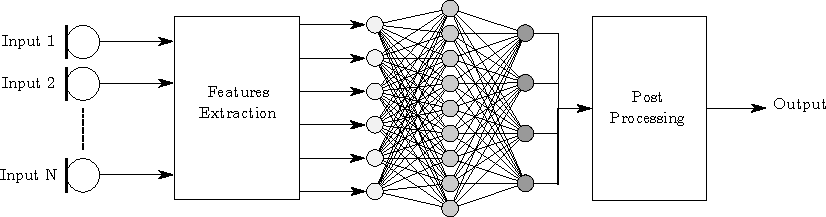
\includegraphics[width=\linewidth]{img/flowchart_1.pdf}
	\caption[Basic structure]{Basic structure of an audio analysis system.}
	\label{fig:base-system}
\end{figure}

\begin{figure}[tb]
	\centering
	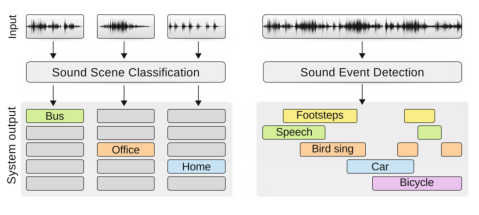
\includegraphics[width=\linewidth]{img/sed_sec.pdf}
	\caption[System input and output ]{System input and output for the two main analysis systems: sound scene classification and sound event detection.}
	\label{fig:system-io}
\end{figure}

The typical computational sound scene
or event analysis system based on machine learning is
depicted in \figref{fig:base-system}, while the different input and output respectively for classification and detection systems
are illustrated in \figref{fig:system-io}.

As the first stage, all the systems take as input one or more audio
signals, either in real-time, captured by a microphone, or offline, from an
audio recording. In this work, we assume always discrete-time signals,
obtained by using analog-to-digital converters. 

The \textit{Feature Extraction} block consists
of different processing stages and outputs acoustic features, as the actual analysis of
audio is rarely based on the raw audio signal, but rather on the compact signal
representation with features. The purpose of the feature extraction is to obtain
information sufficient for detecting or classifying the target sounds, making the
subsequent modeling stage computationally cheaper and also easier to achieve with
limited amount of development material. Very often the feature extraction procedure is also preceded by the down-mixing the audio signal into a single (mono) channel and re-sampling it into fixed sampling frequency.
Although every application could require a specific set of features able to highlight the discriminating particularities of each data sample, the most common representations used
for audio signals are non-linear representation for magnitudes (power spectra and logarithm) and nonlinear frequency scaling (mel-frequency scaling). 
More details of the acoustic features extraction process for each examined case-study will be provided in further chapters.


The \textit{Deep Learning}-based model takes the acoustic features as input and it is trained to produce an output which will assign a class label depending on the application. Almost all the system presented in this work are based on the supervised machine learning approach, where the system is trained using labeled examples of sounds from each of target sound type. 
At the development stage, the obtained acoustic features are used together with
reference annotations of the audio training examples, to learn models for the
sound classes of interest. Annotations contain information about the presence of
target sound classes in the training data, and are used as a reference information
to automatically learn a mapping between acoustic features and class labels. The
mapping is represented by acoustic models. The learning process consists in updating the parameters or \textit{weights} of the neural network, searching for the optimal model that minimize a certain cost-function. 
At the usage stage, the learned acoustic models are used to do recognition (detection or classification), which predicts labels
for the input audio. The recognition stage may also involve temporal models and
post-processing of labels.


After a prediction is obtained through the trained acoustic model, the \textit{Post Processing} stage translates this signal into the effective activity information for each class. Very often this relies on a simple \textit{thresholding} operation or on the selection of the most probable class.



%\subsection{Problem statement} - MOVE TO SED CHAPTER
%The whole system is composed of a feature extraction stage and a detection stage. The feature extraction stage transforms the audio signal into acoustic spectral features, while the second stage processes these features to detect the onset and offset times of specific sound events.
%In this latter stage we include the capsule units. The network parameters are obtained by supervised learning using annotations of sound events activity as target vectors. We have evaluated the proposed method against three datasets of real-life recordings and we have compared its performance both with the results of experiments with a traditional CNN architecture, and with the performance of well-established algorithms which have been assessed on the same datasets.
%
%The aim of polyphonic SED is to find and classify any sound event present in an audio signal. The algorithm we propose is composed of two main stages: sound representation and polyphonic detection. In the sound representation stage, the audio signal is transformed in a two-dimensional time-frequency representation to obtain, for each frame $t$ of the audio signal, a feature vector $\mathbf{x}_t \in \mathbb{R}^F$, where $F$ represents the number of frequency bands. 
%
%Sound events possess temporal characteristics that can be exploited for SED, thus certain events can be efficiently distinguished by their time evolution. Impulsive sounds are extremely compact in time (e.g., gunshot, object impact), while other sound events have indefinite length (i.e., wind blowing, people walking). Other events can be distinguished from their spectral evolution (e.g., bird singing, car passing by). Long-term time domain information is very beneficial for SED and motivates for the use of a temporal \textit{context} allowing the algorithm to extract information from a chronological sequence of input features. Consequently, these are presented as a context window matrix $\mathbf{X}_{t:t+T-1} \in \mathbb{R}^{T \times F \times C}$, where $T\in \mathbb{N}$ is the number of frames that defines the sequence length of the temporal context, $F\in \mathbb{N}$ is the number of frequency bands and $C$ is the number of audio channels. Differently, the target output matrix is defined as $\mathbf{Y}_{t:t+T-1} \in \mathbb{N}^{T \times K}$, where $K$ is the number of sound event classes.
%
%In the SED stage, the task is to estimate the probabilities $p(\mathbf{Y}_{t:t+T-1}| \mathbf{X}_{t:t+T-1},  \boldsymbol{\theta}) \in \mathbb{R}^{T \times K}$, % for the $K$ event classes, %$k = 1,2,\dots,K$
%where $ \boldsymbol{\theta}$ denotes the parameters of the neural network.
%The network outputs, i.e., the event activity probabilities, are then compared with a threshold in order to obtain event activity predictions $\mathbf{\hat{Y}}_{t:t+T-1}  \in \mathbb{N}^{T \times K}$.
%The parameters $ \boldsymbol{\theta}$  are trained by supervised learning, using the frame-based annotation of the sound event class as target output, thus, if class $k$ is active during frame $t$, $Y(t,k)$ is equal to 1, and is set to 0 otherwise. The case of polyphonic SED implies that this target output matrix can have multiple non-zero elements $K$ in the same frame $t$, since several classes can be simultaneously present. 
%
%Indeed, polyphonic SED can be formulated as a multi-label classification problem in which the sound event classes are detected by multi-label annotations over consecutive time frames. The onset and offset time for each sound event are obtained by combining the classification results over consequent time frames. The trained model will then be used to predict the activity of the sound event classes in an audio stream without any further post-processing operations and prior knowledge on the events locations.







\section{State of the Art}


Traditionally, the computational acoustic event analysis has been approached with statistical modelling methods, including Hidden Markov Models (HMM) \cite{degara2011onset}, Gaussian Mixture Models (GMM) \cite{heittola2010audio}, Non-negative Matrix Factorization (NMF) \cite{carabias2011musical} and support vector machines (SVM) \cite{guo2003content}. 

In the recent era of the ``Deep Learning'', different neural network architectures have been successfully used for sound event detection and classification tasks, including feed-forward neural networks (FNN) \cite{mcloughlin2015robust}, deep belief networks \cite{mohamed2012acoustic}, convolutional neural networks (CNNs) \cite{piczak2015environmental} and Recurrent Neural Networks (RNNs) \cite{graves2013speech}. In addition, these architectures laid the foundation for end-to-end systems \cite{trigeorgis2016adieu, wu2017end}, in which the feature representation of the audio input is automatically learnt from the raw audio signal waveforms. 

The use of deep learning models has been motivated by the increased availability of datasets and computational resources and resulted in significant performance improvements, outperforming in most of the cases the human accuracy \cite{sailor2017unsupervised}.
The methods based on CNNs and RNNs have established the new state-of-the-art performance on the sound event detection task (SED), thanks to the capabilities to learn the non-linear relationship between time-frequency features of the audio signal and a target vector representing sound events. In \cite{espi2015}, the authors show how ``local'' patterns can be learned by a CNN and can be exploited to improve the performance of detection and classification of non-speech acoustic events occurring in conversation scenes, in particular compared to a FNN-based system which processes multiple resolution spectrograms in parallel. 

This
success is a result of close academic-industrial collaboration, which started from the speech or speaker recognition task and extended to the analysis of non-speech, music and sound scenes and events. The combination of the CNN structure with recurrent units has increased the detection performance by taking advantage of the characteristics of each architecture. This is the case of convolutional recurrent neural networks (CRNNs) \cite{cakir2017convolutional}, which provided state-of-the-art performance especially in the case of polyphonic SED. CRNNs consolidate the CNN property of local shift invariance with the capability to model short and long term temporal dependencies provided by the RNN layers. This architecture has been also employed in almost all of the most performing algorithms proposed in the last editions of research challenges such as the IEEE Audio and Acoustic Signal Processing (AASP) Challenge on  Detection and Classification of Acoustic Scenes and Events (DCASE) \cite{DCASE2017Workshop}. 

On the other hand, if the datasets are not sufficiently large, problems such as overfitting can be encountered with these models, which typically are composed of a considerable number of free-parameters (i.e., more than 1M). 

Encouraging polyphonic SED performance have been obtained using CapsNets in preliminary experiments conducted on the Bird Audio Detection task in occasion of the DCASE 2018 challenge \cite{vesperini2018capsule}, confirmed by the results reported in \cite{iqbal2018capsule}.
The CapsNet \cite{sabour2017dynamic} is a recently proposed architecture for image classification and it is based on the grouping of activation units into novel structures introduced in \cite{hinton2011transforming}, named \textit{capsules}, along with a procedure called dynamic routing. The capsule has been designed to represent a set of properties for an entity of interest, while dynamic routing is included to allow the network to implicitly learn global coherence and to identify part-whole relationships between capsules.

%TODO move to SED chapter
%The authors of \cite{sabour2017dynamic} show that CapsNets outperform state-of-the-art approaches based on CNNs for digit recognition in the MNIST dataset case study.
%They designed the CapsNet to learn how to assign the suited partial information to the entities that the neural network has to predict in the final classification. This property should overcome the limitations of solutions such as max-pooling, currently employed in CNNs to provide local translation invariance, but often reported to cause an excessive information loss. Theoretically, the introduction of the dynamic routing can supply invariances for any property captured by a capsule, allowing also to adequately train the model without requiring extensive data augmentation or dedicated domain adaptation procedures.


\section{Case studies}
In this work, different application of deep learning for computational audio models in real environments are analyzed. They are evaluated and compared with state-of-the-art methods on different databases, some of these resulting novel approaches. The broad and extensive experimental evaluations highlight the advantages provided by the acoustic models based on deep learning.

The addressed tasks are the following:
\begin{itemize}
	\item Sound event \textit{Classification}:
	\begin{itemize}
		\item Snore sounds excitation localization;
		\item Acoustic road surface roughness classification;
		\item Bird audio detection;
	\end{itemize}
	\item Sound event \textit{Detection}:
	\begin{itemize}
		\item Overnight snore sound detection;
		\item Rare sound event detection;
		\item Polyphonic sound event detection;
		\item Voice activity detection in multiroom environments
	\end{itemize}
\end{itemize}




